\chapter {Interfacing a Light Emitting Diode}
\thispagestyle{empty}
\label{led}
\newcommand{\LocLEDfig}{\Origin/user-code/led/figures}
\newcommand{\LocLEDscicode}{\Origin/user-code/led/scilab}
\newcommand{\LocLEDscibrief}[1]{{\tt \seqsplit{%
        Origin/user-code/led/scilab/#1}}, see \fnrefp{fn:file-loc}}
\newcommand{\LocLEDardcode}{\Origin/user-code/led/arduino}
\newcommand{\LocLEDardbrief}[1]{{\tt \seqsplit{%
        Origin/user-code/led/arduino/#1}}, see \fnrefp{fn:file-loc}}

\newcommand{\LocLEDpycode}{\Origin/user-code/led/python}  %added for python
\newcommand{\LocLEDpybrief}[1]{{\tt \seqsplit{%
        Origin/user-code/led/python/#1}}, see \fnrefp{fn:file-loc}} % added for python


\newcommand{\LocLEDjuliacode}{\Origin/user-code/led/julia}  %added for julia
\newcommand{\LocLEDjuliabrief}[1]{{\tt \seqsplit{%
        Origin/user-code/led/julia/#1}}, see \fnrefp{fn:file-loc}} % added for julia

%%%%%%OpenModelica Starts
\newcommand{\LocLEDOpenModelicacode}{\Origin/user-code/led/OpenModelica}  %added for OpenModelica
\newcommand{\LocLEDOpenModelicabrief}[1]{{\tt \seqsplit{%
        Origin/user-code/led/OpenModelica/#1}}, see \fnrefp{fn:file-loc}} % added for OpenModelica

%%%%%OpenModelcia Ends

In this chapter, we will learn how to control the LEDs on the Shield
and on the \arduino\ board.  We will do this through the Arduino IDE and other open source software tools. 
% We will do this through the Arduino IDE, Scilab scripts, Scilab Xcos, Python, Julia, and OpenModelica.  
These are beginner level experiments,
and often referred to as the \emph{hello world} task of Arduino.
Although simple, controlling LED is a very important task in all
kinds of electronic boards.

\section{Preliminaries}
\label{sec:led-pril}
A light emitting diode (LED) is a special type of semiconductor diode,
which emits light when voltage is applied across its terminals. A
typical LED has 2 leads: Anode, the positive terminal and Cathode, the
negative terminal.  When sufficient voltage is applied, electrons
combine with the holes, thereby releasing energy in the form of
photons.  These photons emit light and this phenomenon is known as
electroluminescence.  The symbolic representation of an LED is shown
in \figref{fig:ledsym}.  Generally, LEDs are capable of emitting
different colours.  Changing the composition of alloys that are
present in LED helps produce different colours.  A popular LED is an
RGB LED that actually has three LEDs: red, green and blue.

\begin{figure}
  \centering
  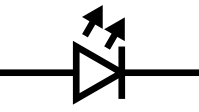
\includegraphics[width=0.2\linewidth]{\LocLEDfig/led.png}
  \caption{Light Emitting Diode}
  \label{fig:ledsym}
\end{figure}

%\subsection{Connection diagram}
An RGB LED is present on the Shield provided in the kit.  In this
section, we will see how to light each of the LEDs present in the RGB
LED.  As a matter of fact, it is possible to create many colours by
combining these three.  A schematic of the RGB LED in the Shield is
given in \figref{fig:ledblock}.
\begin{figure}
  \centering
  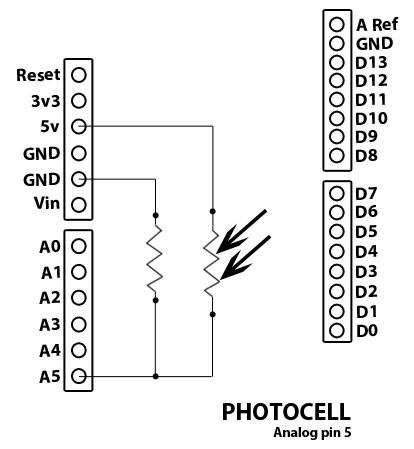
\includegraphics[width=\smfig]{\LocLEDfig/schematic.png}
  \caption{Internal connection diagram for the RGB LED on the Shield}
  \label{fig:ledblock}
\end{figure}
The anode pins of red, green, and blue are connected to pins 11, 10, and 9, 
respectively. Common Cathode is connected to the ground.

It should be pointed out, however, that no wire connections are to be
made by the learner: all the required connections are already made internally 
and it is ready to use.  The LED of any colour can be turned on by
putting a high voltage on the corresponding anode pin.

\begin{figure}
  \centering
  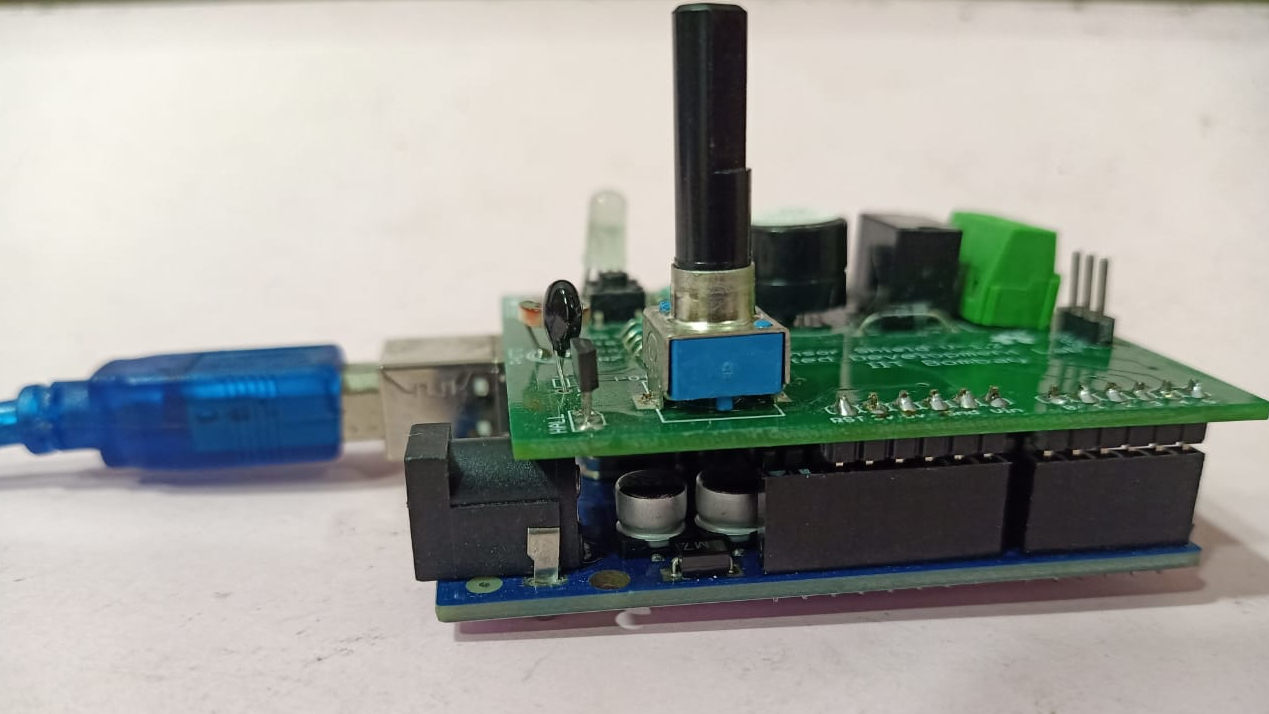
\includegraphics[width=\lgfig]{\LocLEDfig/arduino-new-shield.jpeg}
  \caption{Connecting \arduino\ and Shield}
  \label{fig:uno-shield-connect}
\end{figure}

One should remember to connect the Shield on to the \arduino\ board, as
shown in \figref{fig:uno-shield-connect}. All the experiments in this
chapter assume that the Shield is connected to the \arduino\ board.
It is also possible to do some of the experiments without the Shield,
which is pointed out in the next section. 

\section{Connecting an RGB LED with \arduino\ using a breadboard}
\label{sec:led-bread}
This section is useful for those who either don't have a Shield or don't want to use the Shield
for performing the experiments given in this chapter.

A breadboard is a device for holding the components of a circuit and connecting 
them together. We can build an electronic circuit on a breadboard without doing any 
soldering. To know more about the breadboard and other electronic components, 
one should watch the Spoken Tutorials on Arduino as published on
{\tt https://spoken-tutorial.org/}. Ideally, one should go through all the
tutorials labeled as Basic. However, we strongly recommend the readers should
watch the fifth and sixth tutorials, i.e., {\tt First Arduino Program} and 
{\tt Arduino with Tricolor LED and Push button}.

In case you have an RGB LED and want to connect it with \arduino\ on a breadboard, 
please refer to \figref{fig:ard-rgb-bread}. 
\begin{figure}
  \centering
  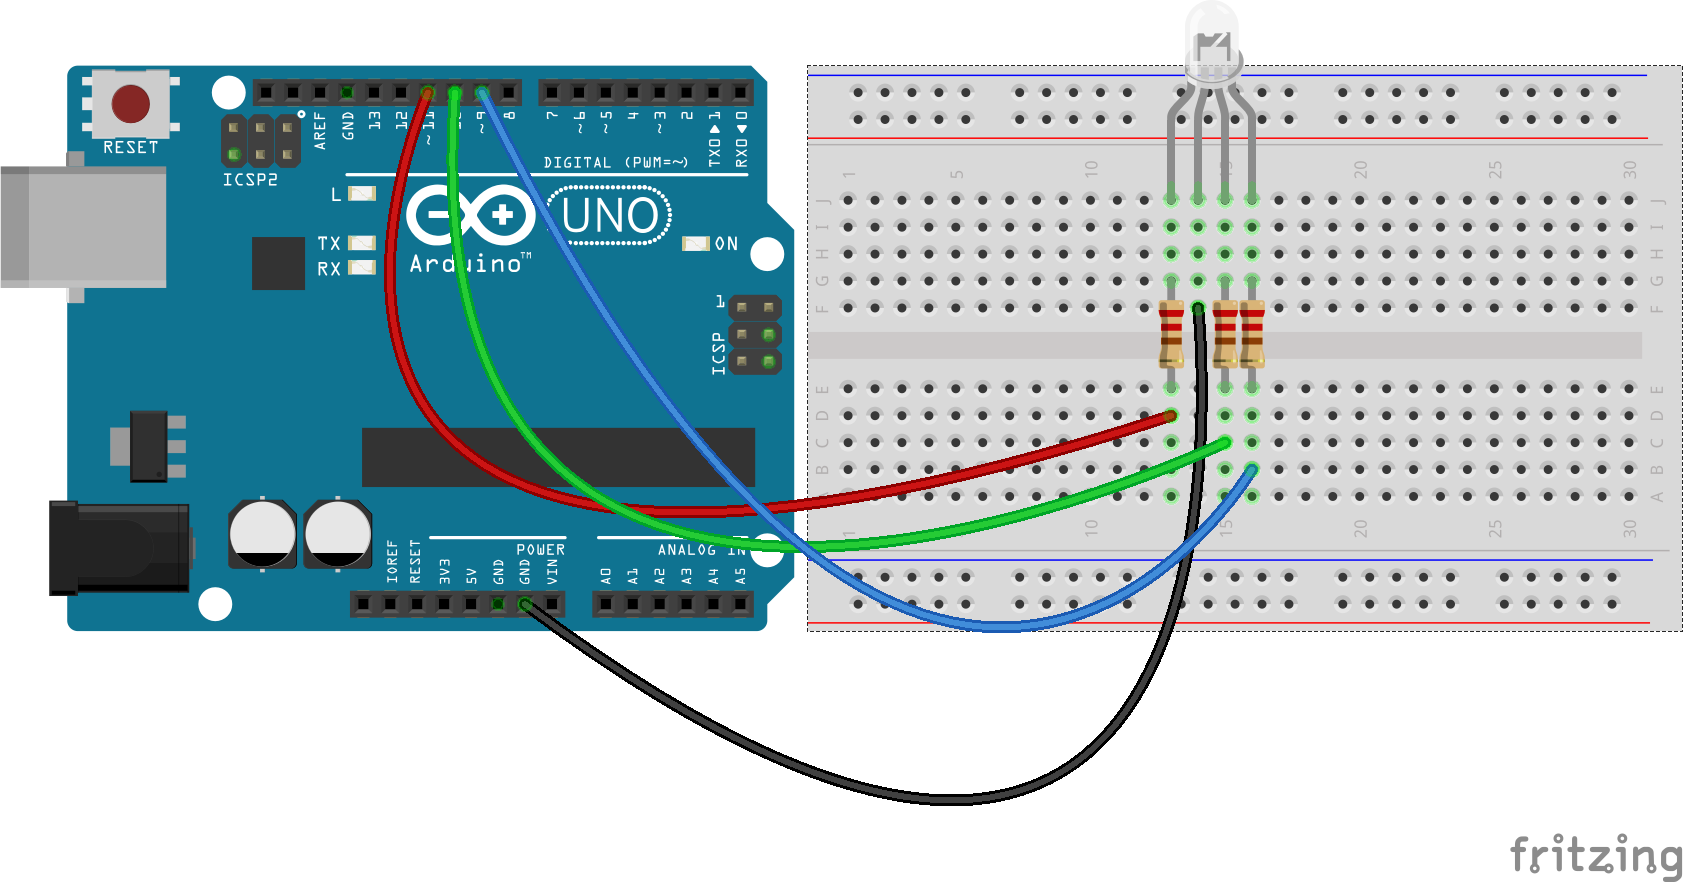
\includegraphics[width=\hgfig]{\LocLEDfig/rgb-led-bb.png}
  \caption{An RGB LED with \arduino\ using a breadboard}
  \label{fig:ard-rgb-bread}
\end{figure}
As shown in \figref{fig:ard-rgb-bread}, there is an RGB LED with four legs. 
From the left, the first leg represents the anode (+) pin for the red LED. 
The second leg represents the common cathode for every color. 
The third and fourth legs represent the anode (+) pins for the green LED and blue LED respectively. 
The anode pins of red, green, and blue are connected to digital pins 11, 10, and 9 of Arduino Uno, respectively. 
Common cathode is connected to the ground (GND) terminal of Arduino Uno. 

\section{Lighting the LED from the Arduino IDE}

\subsection{Lighting the LED}
\label{sec:light-ard}
In this section, we will describe some experiments that will help the
LED light up based on the command given from the Arduino IDE.  We will
also give the necessary code.  We will present four experiments in
this section.  The Shield has to be attached to the \arduino\ board
before doing these experiments and the \arduino\ needs to be connected to the computer 
with a USB cable, as shown in \figref{arduino}. The reader should go through the
instructions given in \secref{sec:ard-start} before getting started.
\begin{enumerate}
  \item First, we will see how to light up the LED in different
        colours.  An extremely simple code is given in \ardref{ard:led-blue}.
        On uploading this code, you can see that the LED on the Shield turns
        blue.  It is extremely easy to explain this code.  Recall from the
        above discussion that we have to put a high voltage (5V) on pin 9 to
        turn the blue light on.  This is achieved by the following command:
        \lstinputlisting[firstline=4,lastline=4]
        {\LocLEDardcode/led-blue/led-blue.ino}
        Before that, we need to define pin 9 as the
        output pin.  This is achieved by the command,
        \lstinputlisting[firstline=2,lastline=2]
        {\LocLEDardcode/led-blue/led-blue.ino}
        One can see that the blue light will be on continuously.  
        
  \item Next, we will modify the code slightly so that the blue light
        remains on for two seconds and then turns off.
        \ardref{ard:led-blue-delay} helps achieve this.  In this, we
        introduce a new command {\tt delay} as below:
        \lstinputlisting[firstline=5,lastline=5]
        {\LocLEDardcode/led-blue-delay/led-blue-delay.ino} This delay
        command halts the code for the time passed as in input argument. In
        our case, it is 2,000 milliseconds, or 2 seconds.  The next command,
        \lstinputlisting[firstline=6,lastline=6]
        {\LocLEDardcode/led-blue-delay/led-blue-delay.ino} puts a low
        voltage on pin 9 to turn it off.
        
        What is the role of the {\tt delay} command?  To find this,
        comment the delay command.  That is, replace the above delay command
        with the following and upload the code.
        \begin{lstlisting}[style=nonumbers]
    // delay(2000);
  \end{lstlisting}
        If you observe carefully, you will see that the LED turns blue
        momentarily and then turns off.
        
  \item We mentioned earlier that it was possible to light more than one
        LED simultaneously.  We will now describe this with another
        experiment.  In this, we will turn on both blue and red LEDs.  We
        will keep both of them on for 5 seconds and then turn blue off,
        leaving only red on.  After 3 seconds, we will turn red also off.
        This code is given in \ardref{ard:led-blue-red}.  Remember that
        before writing either {\tt HIGH} or {\tt LOW} on to any pin, its
        mode has to be declared as {\tt OUTPUT}, as given in the code.  All
        the commands in this code are self explanatory.
        
  \item Finally, we will give a hint of how to use the programming
        capabilities of the Arduino IDE.  For this, we will use
        \ardref{ard:led-blink}.  It makes the LED blink 5 times.  Recall
        from the previous section that a {\tt HIGH} on pin 10 turns on the
        green LED.  This cycle is executed for a total of five times.  In each
        iteration, it will turn the green LED on for a second by giving the
          {\tt HIGH} signal and then turn it off for a second by giving the
          {\tt LOW} signal.  This cycle is carried out for a total of 5 times,
        because of the {\tt for} loop.
\end{enumerate}

\paragraph{Note:}
All the above four experiments have been done with
the Shield affixed to the \arduino\ board.  One may run these
experiments without the Shield as well.  But in this case, pin number
13 has to be used in all experiments, as pin 13 lights up the LED that
is on the \arduino\ board.  For example, in \ardref{ard:led-blue}, one
has to replace both occurrences of number 9 with 13.  In this case,
one will get the LED of \arduino\ board light up, as shown in
\figref{fig:led-uno}.
\begin{figure}
  \centering
  \includegraphics[width=\hgfig]{\LocLEDfig/led_output.png}
  \caption{LED experiments directly on \arduino\ board, without the
    Shield}
  \label{fig:led-uno}
\end{figure}


\paragraph{Note:} It should also be pointed out that only one colour
is available in \arduino\ board.  As a result, it is not possible to
conduct the experiments that produce different colours if the
Shield is not used.

\begin{exercise}
  Carry out the following exercise:
  \begin{enumerate}
    \item In \ardref{ard:led-blue-delay}, remove the delay, as discussed
          above, and check what happens.
    \item Light up all three colours simultaneously, by modifying
          \ardref{ard:led-blue-red}.  Change the
          combination of colours to get different colours.
    \item Incorporate some of the features of earlier experiments into
          \ardref{ard:led-blink} and come up with different ways of blinking
          with different colour combinations.
  \end{enumerate}
\end{exercise}

\subsection{Arduino Code}
\lstset{style=mystyle}
\label{sec:led-arduino-code}
\addtocontents{ard}{\protect\addvspace{\codclr}}

\begin{ardcode}
  \acaption{Turning on the blue LED}{Turning on the blue LED.  Available
    at \LocLEDardbrief{led-blue/led-blue.ino}.}
  \label{ard:led-blue}
  \lstinputlisting{\LocLEDardcode/led-blue/led-blue.ino}
\end{ardcode}

\begin{ardcode}
  \acaption{Turning on the blue LED and turning it off after two
    seconds}{Turning on the blue LED and turning it off after two
    seconds.  Available  
    at \LocLEDardbrief{led-blue-delay/led-blue-delay.ino}.}
  \label{ard:led-blue-delay}
  \lstinputlisting{\LocLEDardcode/led-blue-delay/led-blue-delay.ino}
\end{ardcode}

\begin{ardcode}
  \acaption{Turning on blue and red LEDs for 5 seconds and then turning
    them off one by one}{Turning on blue and red LEDs for 5 seconds and
    then turning them off one by one.  Available at
    \LocLEDardbrief{led-blue-red/led-blue-red.ino}.}
  \label{ard:led-blue-red}
  \lstinputlisting{\LocLEDardcode/led-blue-red/led-blue-red.ino}
\end{ardcode}

\begin{ardcode}
  \acaption{Blinking the green LED}{Blinking the green LED.  Available
    at \LocLEDardbrief{led-green-blink/led-green-blink.ino}.}
  \label{ard:led-blink}
  \lstinputlisting{\LocLEDardcode/led-green-blink/led-green-blink.ino}
\end{ardcode}


